%\documentclass[tikz, border=5pt]{standalone}
\begin{document}
	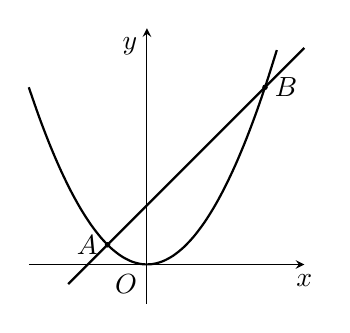
\begin{tikzpicture}[>=stealth, scale=0.5]
		% 1. 绘制坐标轴
		\draw[->] (-3, 0) -- (4, 0) node[below] {$x$};
		\draw[->] (0, -1) -- (0, 6) node[below left] {$y$};
		\node at (0, 0) [below left] {$O$};  % 标记原点
		
		% 2. 绘制抛物线 \( 2y = x^2 \)(即 \( y = \frac{x^2}{2} \))
		\draw[thick, domain=-3:3.3, smooth, variable=\x]
		plot (\x, {\x*\x / 2});
		
		% 3. 绘制直线 \( y = x + 1.5 \)
		\draw[thick, domain=-2:4]
		plot (\x, {\x + 1.5});
		
		% 4. 标记交点 \( A(-1, 0.5) \) 和 \( B(3, 4.5) \)
		\fill (-1, 0.5) circle (2pt) node[ left] {$A$};
		\fill (3, 4.5) circle (2pt) node[ right] {$B$};
	\end{tikzpicture}
\end{document}
